\section*{Question 3:}
Exercise 10.6: 

Find two examples of document filtering systems on the Web. How do they build a profile for your information need? Is the system static or adaptive?


\subsection*{Answer:}

For my two examples I have chosen Amazon and Youtube. Both of them use an adaptive system for making recommendations. 

Amazon is an e-commerce company. I use it sometimes to purchase different items including car parts, electronics, and other items. The screen shot below shows recommended items for me based on items that I viewed, fuel pumps, and items I purchased recently, a cable to connect my truck to my laptop and perform different diagnosis and scanning. Other recommended items are products that were viewed or bought by people whose purchase history is similar to mine. Amazon does such a good job as far as recommendations. I would buy all the recommended items if I had enough money to splurge. 

\begin{figure}[h]
\caption{Recommended items by Amazon}
\centering
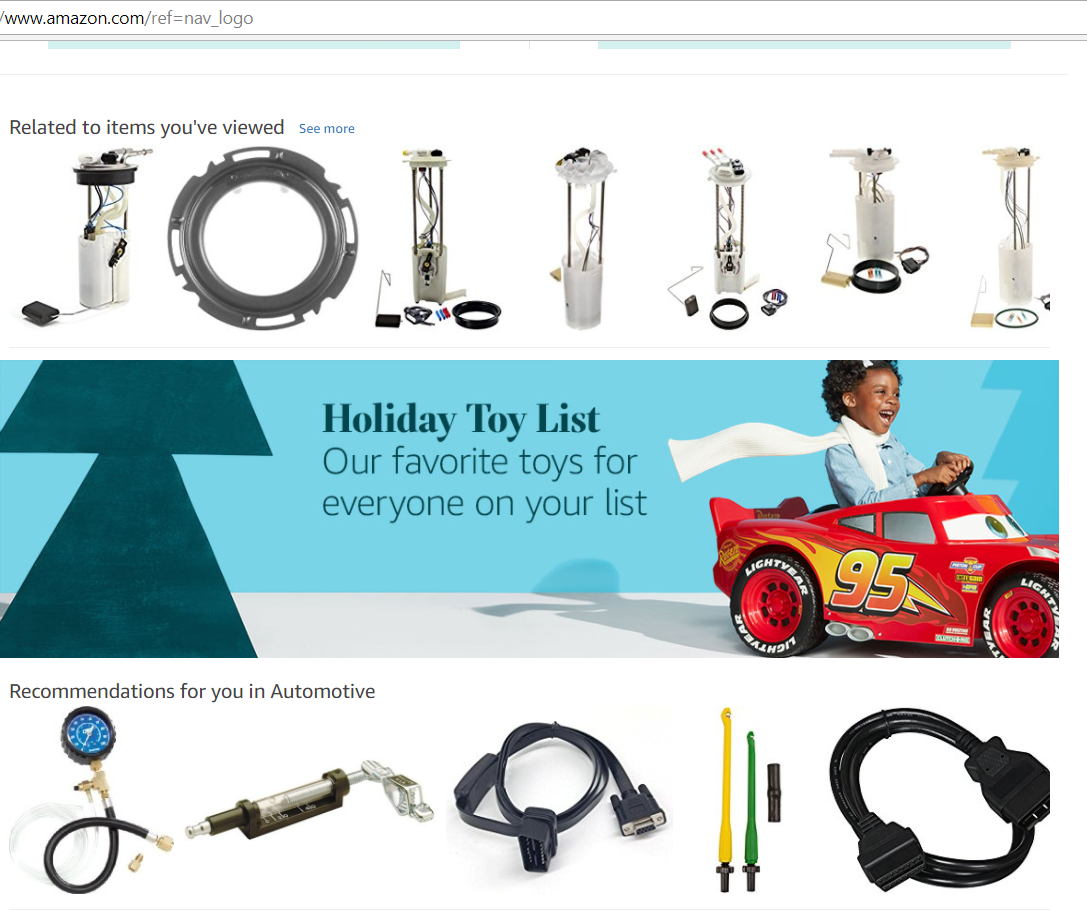
\includegraphics[scale=0.6]{Q3/amazon.png}
\end{figure}

\pagebreak

Youtube is my favorite website. The reason is that I use it for everything including entertainment, news, music, nutrition, and fitness videos. I also watch short lectures or tutorials about concepts I do not understand in Computer Science. Youtube recommends videos for me based on other videos I watched. It also recommends channels/users for me to subscribe to based on videos I watched or other channels I am subscribed to. It also shows popular uploads from channels I am subscribed to.

The screen shot below shows a list of recommended videos, based on videos I watched recently. The recommended videos belong to different categories including entertainment, news, music, fitness, boxing, UFC, ...etc.

\begin{figure}[h]
\caption{Recommended items by Youtube}
\centering
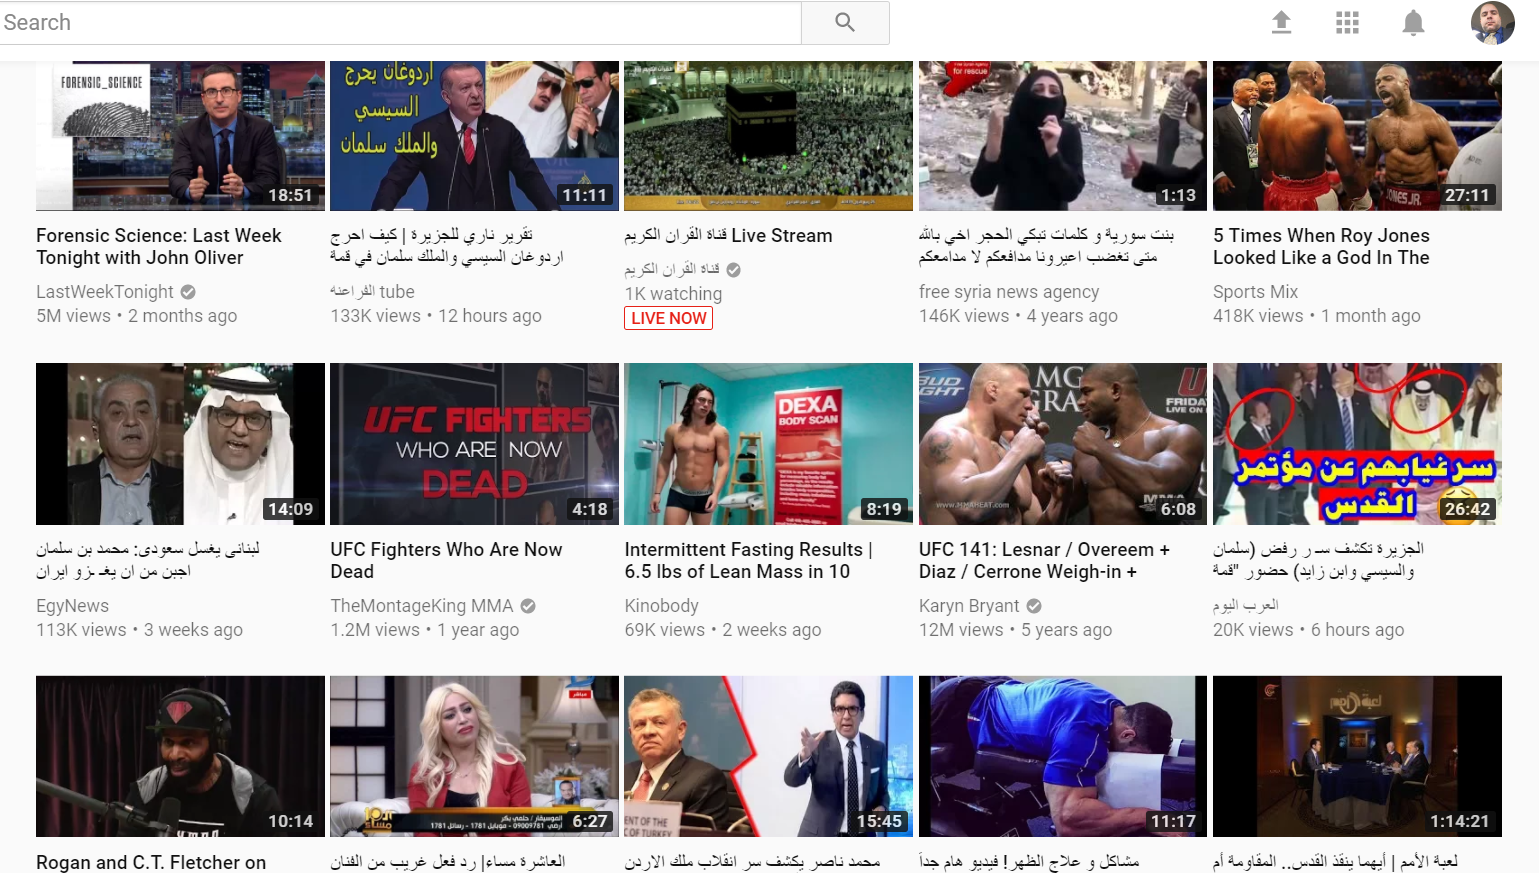
\includegraphics[scale=0.45]{Q3/yrv.png}
\end{figure}

\pagebreak

The screen shot below shows a list of popular uploads from a nutrition channel I am subscribed to, Dr. Josh Axe, as well as a recommended channel for my to subscribe to based on videos I watched and channels I am subscribed to. The recommended channel is an Arabic media channel that posts news from the middle east and other videos about politics.

\begin{figure}[h]
\caption{Recommended items by Youtube}
\centering
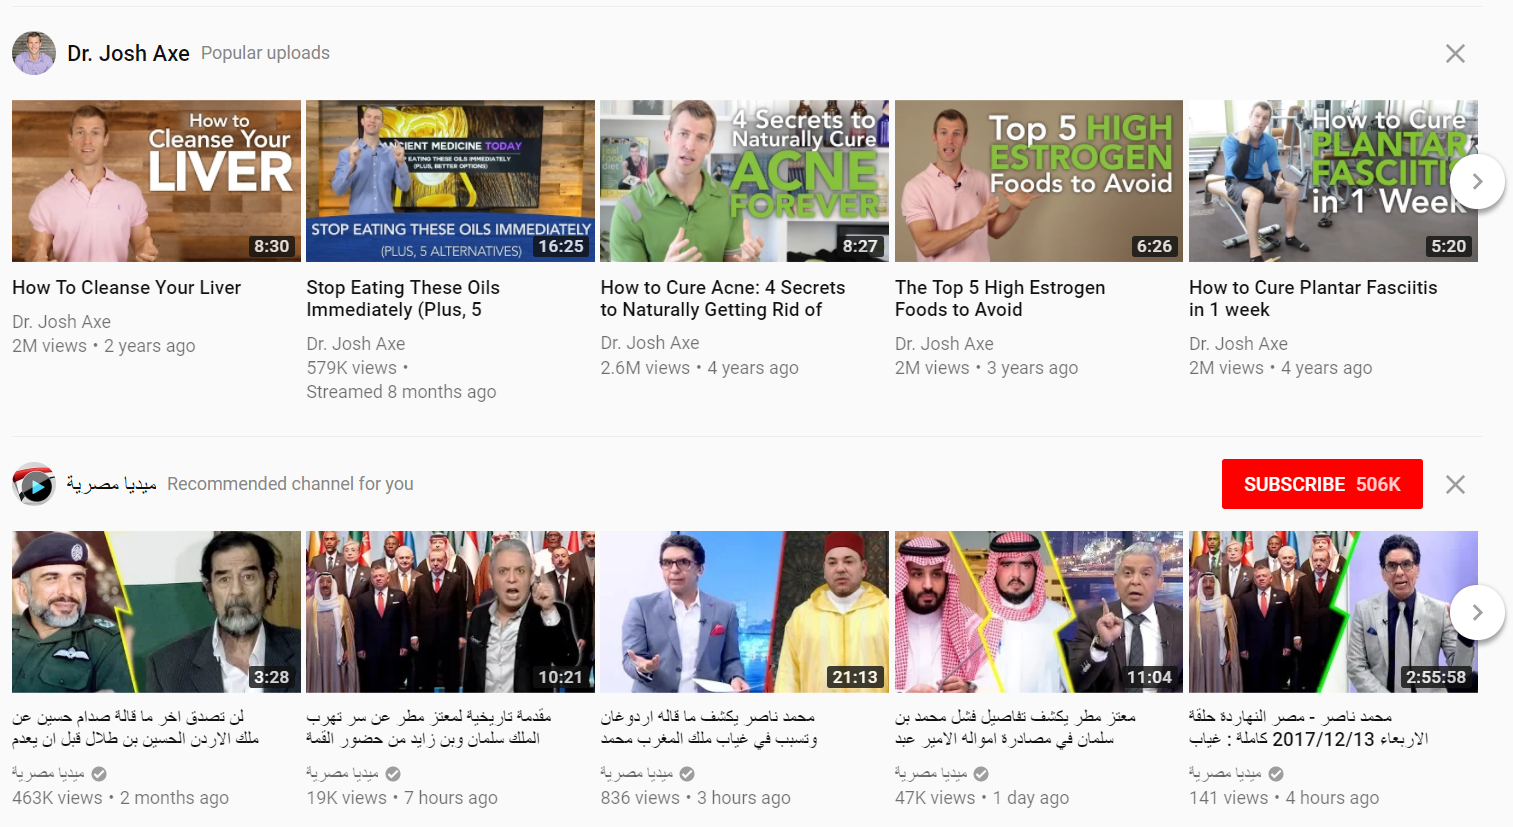
\includegraphics[scale=0.45]{Q3/yrc.png}
\end{figure}

\pagebreak

Youtube also shows a list of videos that I did not complete in case I wanted to continue to watch them. It also shows a list of recently uploaded videos that belong to categories in which I am interested based on my views history as the screen shot below shows.

\begin{figure}[h]
\caption{Recommended items by Youtube}
\centering
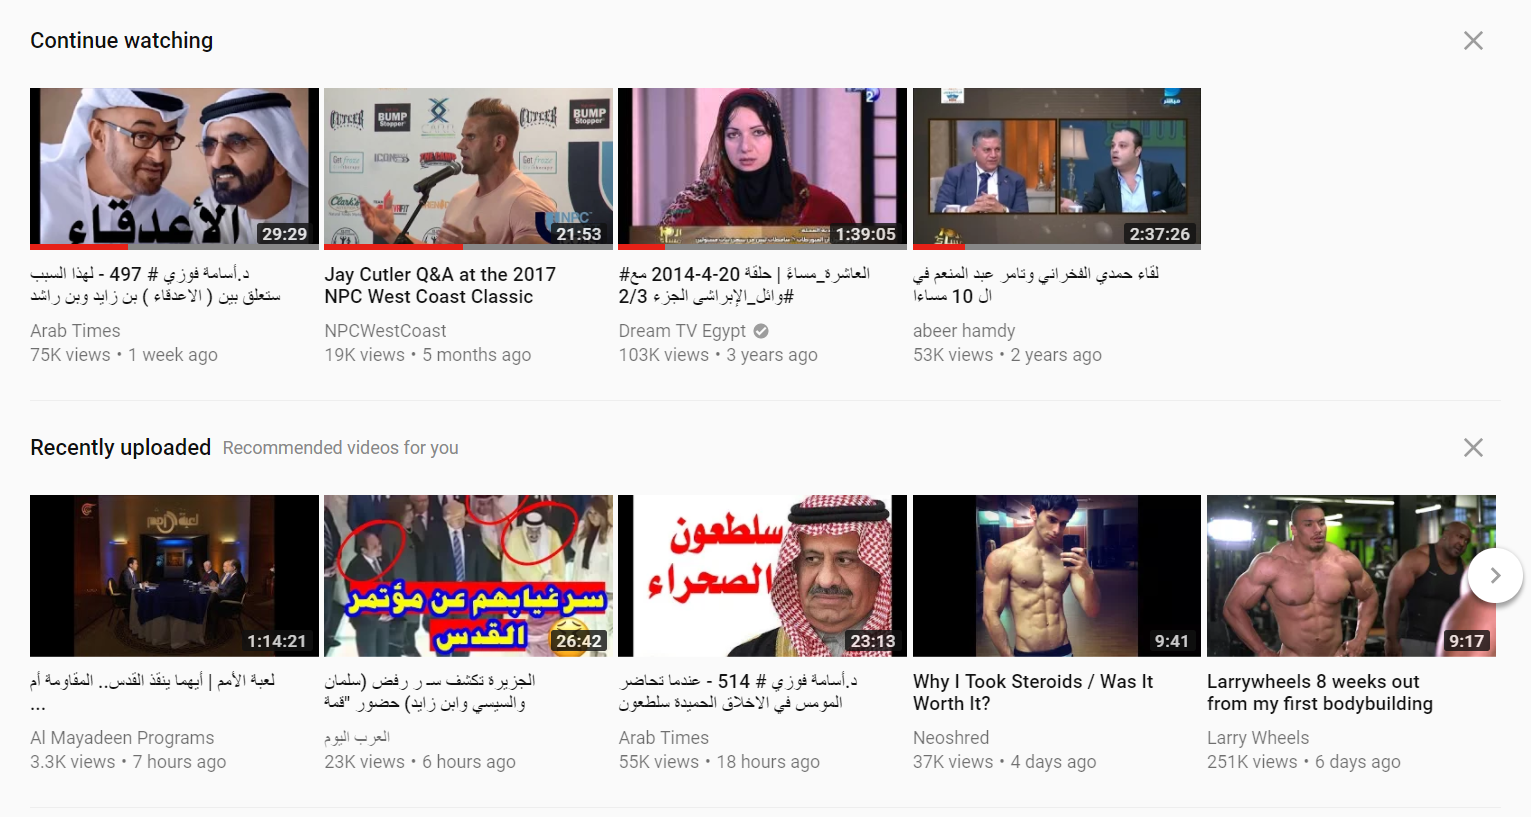
\includegraphics[scale=0.45]{Q3/yrr.png}
\end{figure}

\pagebreak

Youtube shows a list of live recommendations based on live channels I watch, mostly news. It also shows recommended a nonstop playlists ,Youtube mixes, based on a song or an atrist from my views history. I turned off recommended videos from one of the channels I am not interested in, RT Arabic. Youtube says: Got it. We'll tune your recommendations. It gave me the option to undo in case my cat turned that recommendation off for me. The screen shot below shows what I described.


\begin{figure}[h]
\caption{Recommended items by Youtube}
\centering
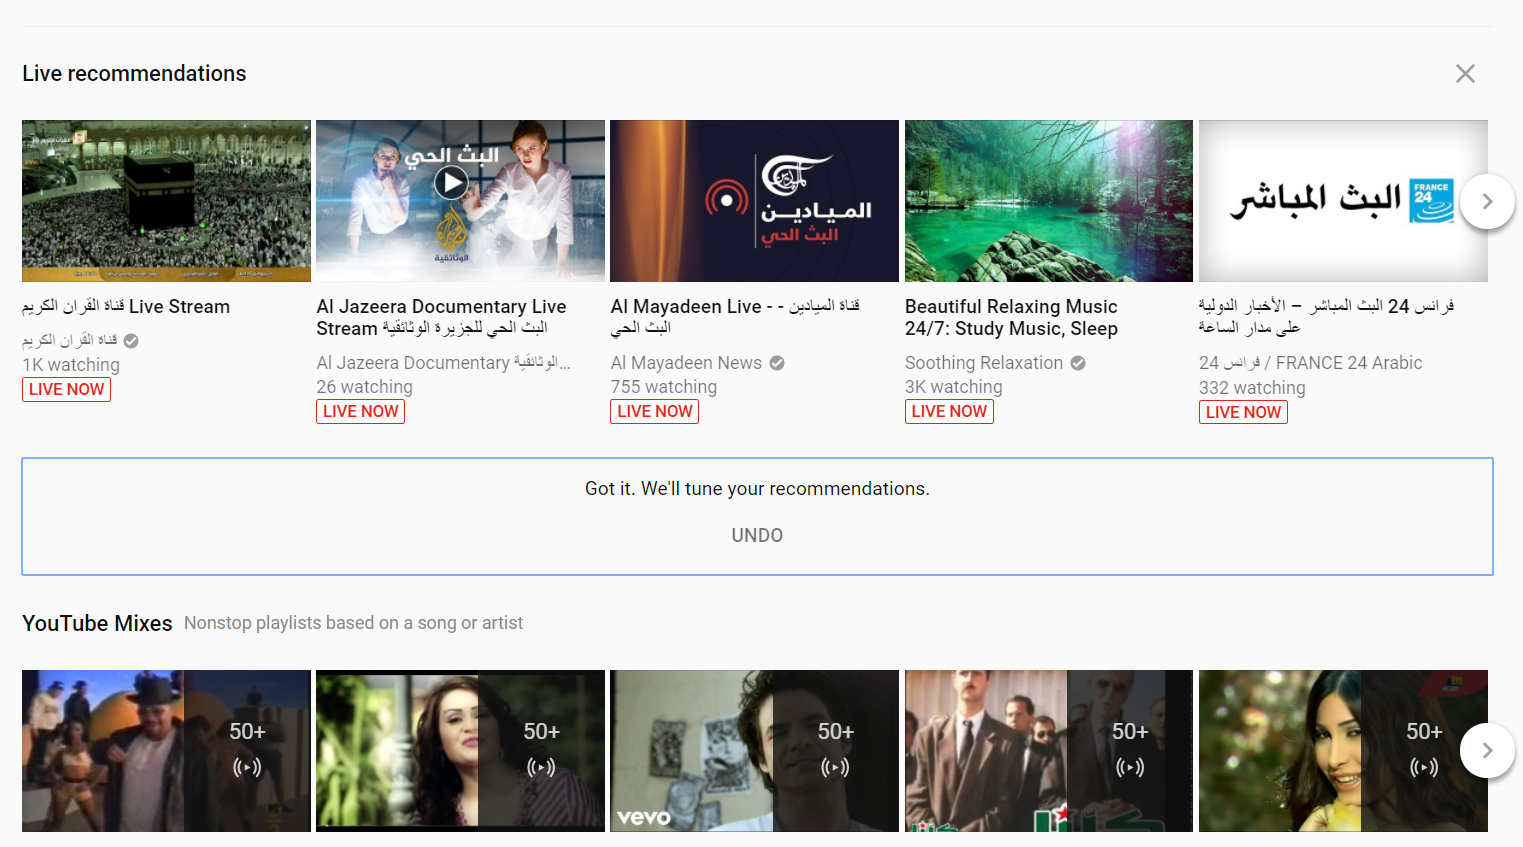
\includegraphics[scale=0.45]{Q3/yrp.png}
\end{figure}

\pagebreak

So far, it seems like Youtube is recommending the right videos for me, however, it also shows videos I am not interested in. This could be because these videos have so many views, millions, as seen in the next screen shot. I am not interested in Trailers, but Youtube shows it anyways.

\begin{figure}[h]
\caption{Recommended items by Youtube}
\centering
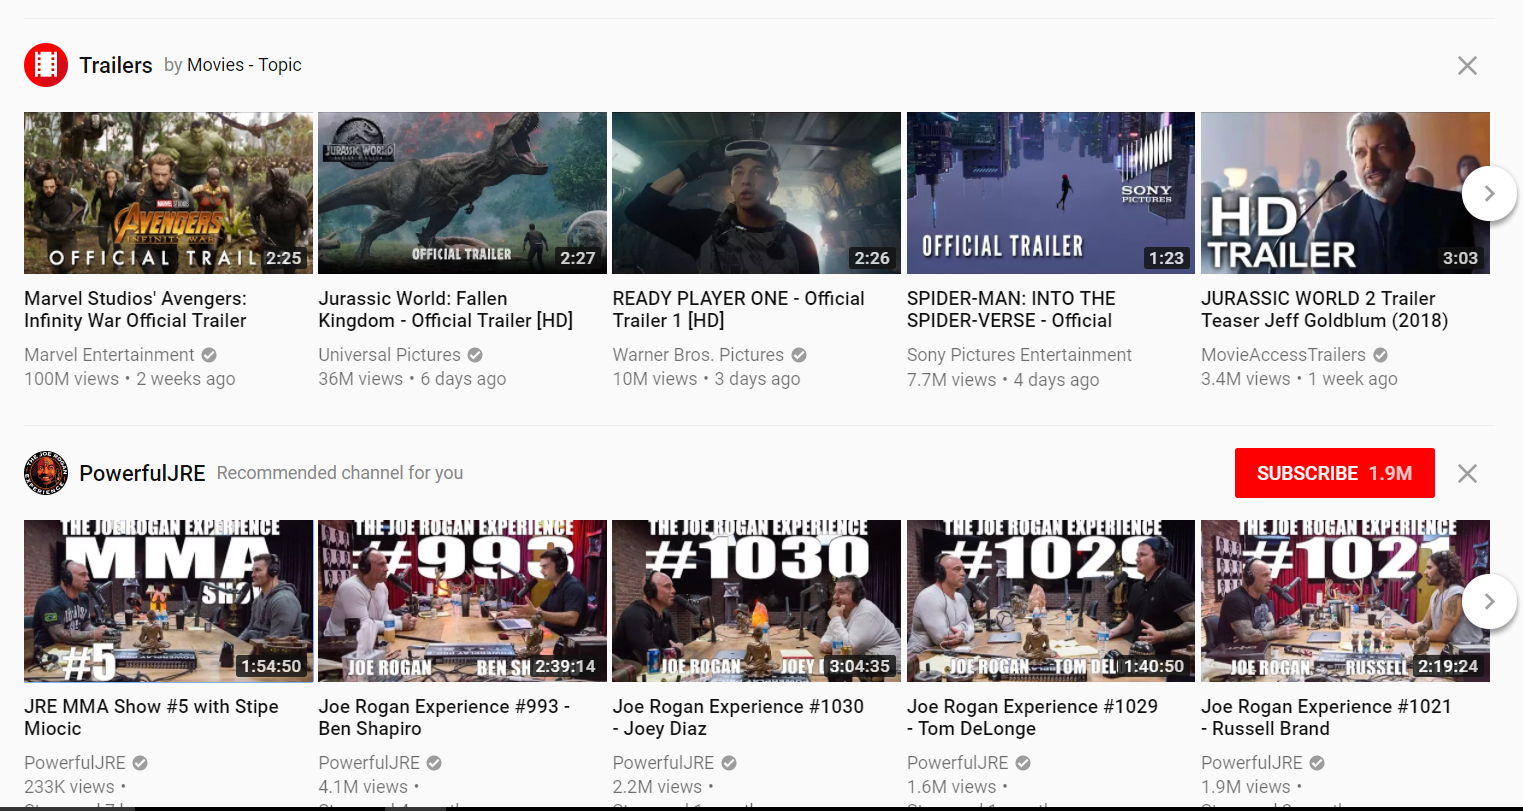
\includegraphics[scale=0.45]{Q3/yrt.png}
\end{figure}

\pagebreak

Finally, Youtube places an ad, sponsored video, in the upper right corner on  video pages I watch. The users who made these videos pay Youtube to show these videos to users based on the video that is on the same page. I have AdBlock installed on my browser so I do not have to see all kinds of advertisements. I disabled AdBlock to take the screen shot below.

\begin{figure}[h]
\caption{Recommended items by Youtube}
\centering
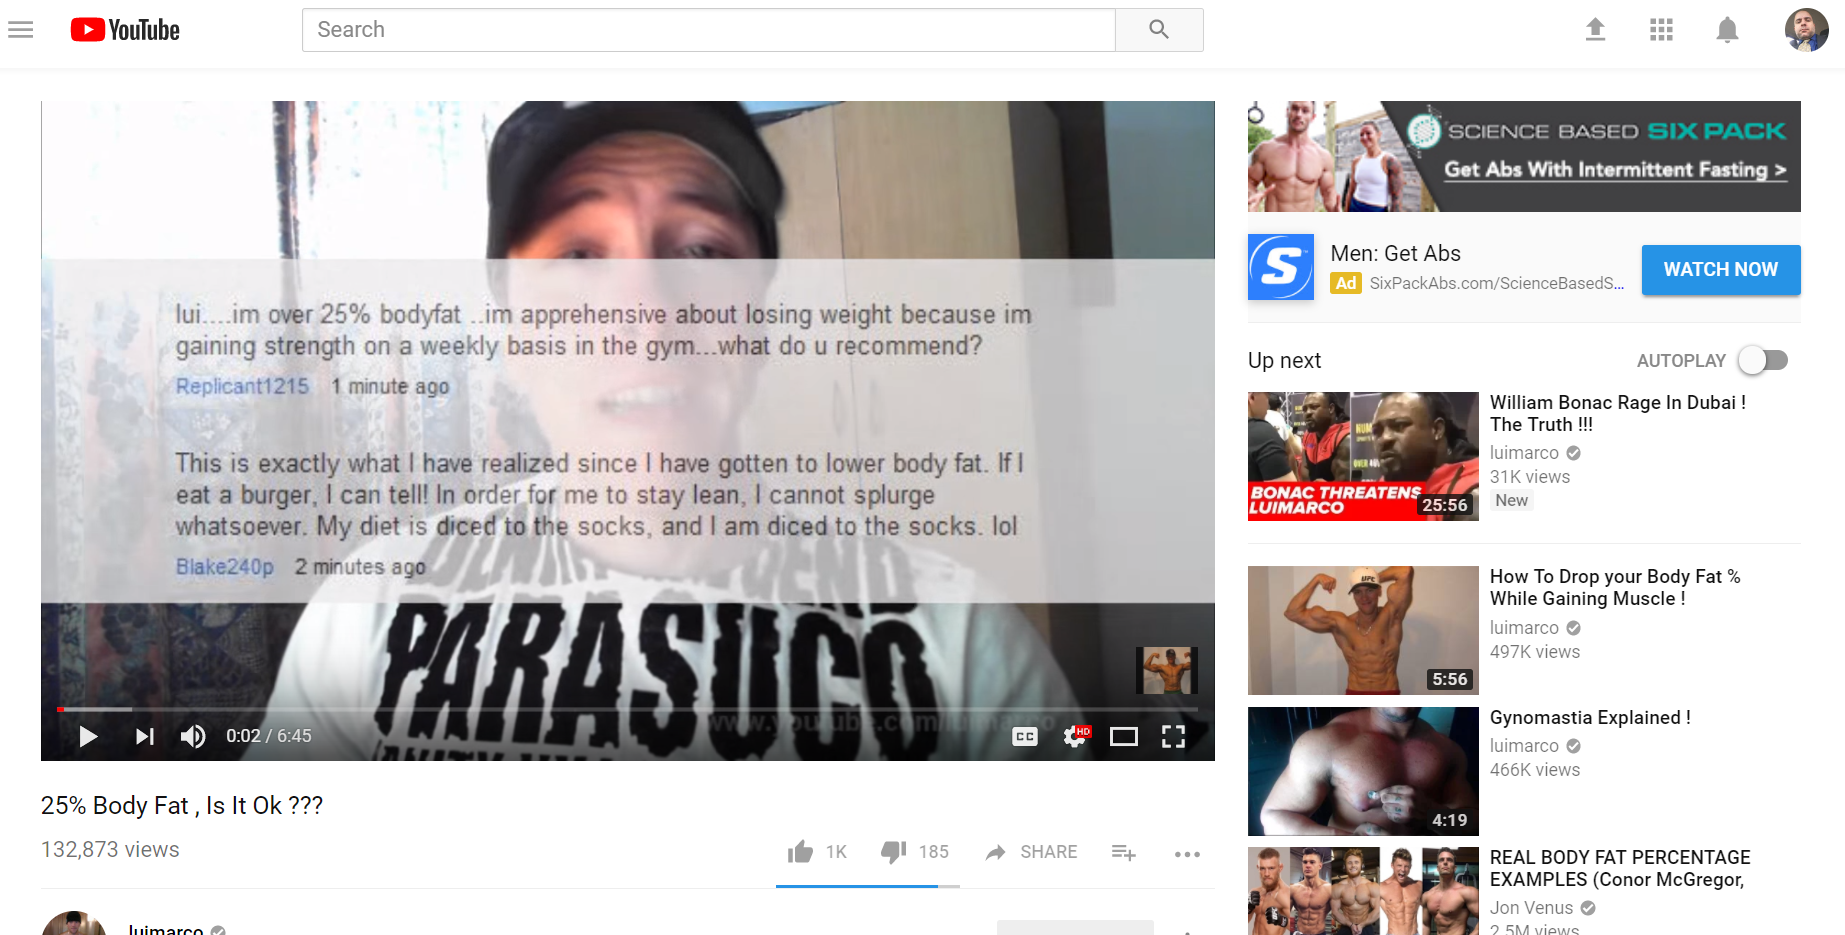
\includegraphics[scale=0.37]{Q3/yrs.png}
\end{figure}
 

 

